\subsubsection{Varying $c_L$ and $c_R$ while fixing $a_L = a_R = 6$, $b_L = -\frac{1}{2}$, and $b_R = -\frac{7}{2}$}

Choosing to make the parabolas centered was not ideal.
When looking at the original model function, one can see that the parabolas are not centered.
All branches are more skewed to the right.
To imitate this shape better, we now set $b_L = -\frac{1}{2}$ and $b_R = -\frac{7}{2}$.
All other fixed parameters are the same as above.
The parameters $c_L$ and $c_R$ are varied in the intervals $[0.08, 0.525]$ and $[0.825, 1.275]$, respectively, to capture a full structure.
\Cref{fig:setup.quad.even.period.full} shows a 2D scan of the periods of the stable cycles in this parameter range.
The structure seen in this figure repeats in all directions.

An interesting parameter area is marked with a red rectangle.
In this parameter area, 2 wings with the same period connect.
\Cref{fig:setup.quad.skew.period.zoomed} shows the 2D scan of the periods for this parameter range.
The points indicate the parameter values for the cobweb analysis.

\begin{figure}
	\centering
	\begin{subfigure}{0.4\textwidth}
		\centering
		\includegraphics[width=\textwidth]{21_Quadratic_mod1/Skew/S_2D_Period_Zoomed1/result.png}
		\caption{Full}
		\label{fig:setup.quad.skew.period.full}
	\end{subfigure}
	\begin{subfigure}{0.4\textwidth}
		\includegraphics[width=\textwidth]{21_Quadratic_mod1/Skew/S_2D_Period_Zoomed2/result.png}
		\caption{Zoomed}
		\label{fig:setup.quad.skew.period.zoomed}
	\end{subfigure}
	\caption[2D scans showing periods of the skewed piecewise quadratic model]{
		2D scans showing the periods of the piecewise quadratic model with fixed parameters $a_L = a_R = 6$, $b_L = -\frac{1}{2}$, and $b_R = -\frac{7}{2}$.
		(a) Shows the full structure with parameters $c_L$ and $c_R$ being varied in the ranges $[0.08, 0.525]$ and $[0.825, 1.275]$, respectively.
		The red rectangle marks the parameter range of (b).
		The marked points in (b) are the parameter values for the cobwebs in \Cref{fig:setup.quad.skew.cobwebs}
	}
	\label{fig:setup.quad.skew.period}
\end{figure}

\begin{figure}
	\centering
	\begin{subfigure}{0.3\textwidth}
		\centering
		\includegraphics[width=\textwidth]{21_Quadratic_mod1/Skew/S_Cobweb_A/result.png}
		\caption{At point $A$}
		\label{fig:setup.quad.skew.cobweb.A}
	\end{subfigure}
	\begin{subfigure}{0.3\textwidth}
		\centering
		\includegraphics[width=\textwidth]{21_Quadratic_mod1/Skew/S_Cobweb_B/result.png}
		\caption{At point $B$}
		\label{fig:setup.quad.skew.cobweb.B}
	\end{subfigure}
	\begin{subfigure}{0.3\textwidth}
		\centering
		\includegraphics[width=\textwidth]{21_Quadratic_mod1/Skew/S_Cobweb_C/result.png}
		\caption{At point $C$}
		\label{fig:setup.quad.skew.cobweb.C}
	\end{subfigure}
	\caption[Cobwebs of the skewed piecewise quadratic model]{
		Cobweb diagrams at three parameter values of $c_L$ and $c_R$ in the piecewise quadratic model with fixed parameters $a_L = a_R = 6$, $b_L = -\frac{1}{2}$, and $b_R = -\frac{7}{2}$.
		The parameter values are marked in \Cref{fig:setup.quad.even.period.zoomed}.
	}
	\label{fig:setup.quad.skew.cobwebs}
\end{figure}

\Cref{fig:setup.quad.skew.cobwebs} shows all the cobwebs taken at the points marked in \Cref{fig:setup.quad.skew.period.zoomed}.
The cobweb at point $A$ is shown in \Cref{fig:setup.quad.skew.cobweb.A}.
We can see that it has period 12 and its symbolic sequence is $\A^4\B^2\C^4\D^2$.
The cycle at point $C$ also has period 12.
Its cobweb diagram is shown in \Cref{fig:setup.quad.skew.cobweb.C}, and we can see that its symbolic sequence is $\A^3\B^3\C^3\D^3$.

From point $A$ to point $C$, one point of the cycle on the branch $f_\A$ moved to the branch $f_\B$.
The same thing happened to a point of the cycle on the branch $f_\C$, it moved to the branch $f_\D$.
This is similar to what happens in the original model along a chain of parameter regions with the same period.
And in between both points, there is a parameter region where 2 cycles coexist.
This is shown in \Cref{fig:setup.quad.skew.cobweb.B}, which depicts the cycles at point $C$.
But unfortunately, the coexisting cycles are the same cycles that exist at point $A$ and point $C$, $\Cycle{\A^4\B^2\C^4\D^2}$ and $\Cycle{\A^3\B^3\C^3\D^3}$.
Similarly to the previous attempt, we merely observe two parameter regions with stable cycles overlapping.
